%% Pour voir les accents de ce fichier, assurez-vous que votre
%% éditeur de texte lise le fichier en utf-8!

%% La classe <dms> est construite au-dessus de <amsbook>, donc
%% <amsmath>, <amsfonts> et <amsthm> sont automatiquement chargés.
\documentclass[12pt,initial,twoside,maitrise]{dms}
\usepackage[utf8]{inputenc} %Obligatoires
\usepackage[T1]{fontenc}    %

\usepackage{xcolor}
\usepackage{listings}
\lstset{basicstyle=\ttfamily,
  columns=fullflexible,
  keepspaces=true,}

\francais %Pour un document en français ou
%\anglais{}

%% Il n'est pas nécessaire d'utiliser <babel>, car
%% les commandes intégrées par la classe <dms>
%% \francais et \anglais font le travail. Néanmoins,
%% certains autres packages nécessitent <babel> (comme
%% <natbib>), donc simplement enlever les % devant <babel>
%% dans ce cas. Attention! Certains packages sont sensibles
%% à l'ordre dans lequel ils sont chargés.
%%
\usepackage[english,frenchb]{babel}

%% La commande \sloppy peut avoir des effets étranges sur les
%% lignes de certains paragraphes.  Dans ce cas, essayez \fussy
%% qui suppresse les effets de \sloppy.
%% (\fussy est normalement le comportement par défaut.)
%% On redéfinit \sloppy, pour tenter de réduire les comportements
%% étranges. Le seul changement apporté à la version originale
%% est la valeur de \tolerance.
\def\sloppy{%
  \tolerance500%  %9999 dans LaTeX ordinaire, mauvaise idée.
  \emergencystretch3em
  \hfuzz.5pt
  \vfuzz\hfuzz}
\sloppy   %appel de \sloppy pour le document
%%\fussy  %ou \fussy
%%
%% Packages utiles.
%%
\usepackage{graphicx,amssymb,subfigure,icomma}
%% icomma       permet d'écrire les nombres décimaux en
%%                  français (p.ex. 1,23 plutôt que 1.23)
%% subfigure    simplifie l'inclusion de figures côtes-à-côtes

%% Packages parfois utiles.
%%\usepackage{dsfont,mathrsfs,color,url,verbatim,booktabs}
%% dsfont       symboles mathématiques \mathds
%% mathrsfs     plus de symboles mathématiques \mathscr
%% color        pour utiliser des couleurs (comparer avec <xcolor>)
%% url          permet l'écriture d'url
%% verbatim     pour écrire du code ou du texte tel quel
%% booktabs     plus de macros pour faire les tableaux
%%                  (voir documentation du package)

%% pour que la largeur de la légende des figures soit = \textwidth
\usepackage[labelfont=bf, width=\linewidth]{caption}

%% les 3 lignes suivante servent à l'affichage de l'index
%% dans le visionneur de pdf. <hyperref> et <bookmark>
%% devraient être les dernier package a être chargé,
%% donc chargez vos packages avant.
\usepackage{hyperref}  % Ajoute les hyperlien
\hypersetup{colorlinks=true,allcolors=black}
\usepackage{hypcap}   % Corrige la position du lien pour les images
\usepackage{bookmark} % Remédie à des petits problème
                      % de <hyperref> (important qu'il
                      % apparaisse APRÈS <hyperref>)

  % Enlever les commentaires du prochaine \hypersetup et
  % le remplir avec l'information pertinente.
  % Ceci ajoute des « méta-données » au pdf.  C'est optionnel,
  % mais recommandé. Vous pouvez voir ces méta-données en
  % ouvrant un visionneur de pdf et en cherchant les propriétés
  % du pdf. (Vous pouvez aussi tapez ' pdfinfo <nom-du-pdf> '
  % dans un terminal.) Ces données sont utiles, par exemple,
  % pour augmenter les chances qu'un algorithme de recherche
  % trouve votre document sur Internet, une fois diffusé.
%%\hypersetup{
%%  pdftitle = {Titre de la thèse / du mémoire},
%%  pdfauthor = {auteur},
%%  pdfsubject = {Ex: Transformation de Fourier ; régressions linéaires ; ... },
%%  pdfkeywords = {Ex: mathématiques, statistiques, groupes, variables aléatoires,...}
%%}

%% Définition des environnements utiles pour un mémoire scientifique.
%% La numérotation est laissée à la discrétion de l'auteur. L'exemple
%% illustré ici produit « Définition x.y.z »
%%   x = no. chapitre
%%   y = no. section
%%   z = no. définition
%%
%% Les macros \<type>name sont telles qu'ils suivent
%% la langue actuelle. (P.ex. si \francais est utilisé,
%% alors \begin{theo} va faire un Théorème et si \anglais
%% est utilisé, \begin{theo} fera un Theorem.)
%%
\newtheorem{cor}{\corollaryname}[section]
\newtheorem{deff}[cor]{\definitionname}
\newtheorem{ex}[cor]{\examplename}
\newtheorem{lem}[cor]{\lemmaname}
\newtheorem{prop}[cor]{Proposition}
\newtheorem{rem}[cor]{\remarkname}
\newtheorem{theo}[cor]{\theoremname}
%% NOTE : Il peut être commode de redéfinir \the<type> pour
%% obtenir la numérotation désirée. Par exemple, pour
%% que les corollaires soit numérotés #section.#sous-section.#sous-sous-section.#paragraphe.#corollaire,
%% on fait
%% \renewcommand\thecor{\theparagraph.\arabic{cor}}

%%%
%%% Si vous préférez que les corollaires, définitions, théorèmes,
%%% etc. soient numérotés successivement, utilisez plutôt un bloc de
%%% commandes de la forme :
%%%
\newcommand\TODO[1]{\colorbox{red}{#1}}
%% \newtheorem{cor}{\corollaryname}[section]
%% \newtheorem{deff}[cor]{\definitionnamr}
%% \newtheorem{ex}[cor]{\examplename}
%% \newtheorem{lem}[cor]{\lemmaname}
%% \newtheorem{prop}[cor]{Proposition}
%% \newtheorem{rem}[cor]{\remarkname}
%% \newtheorem{theo}[cor]{\theoremname}

%%
%% Numérotation des équations par section
%% et des  tableaux et figures par chapitre.
%% Ceci peut être modifié selon les préférences de l'utilisateur.
\numberwithin{equation}{section}
\numberwithin{table}{chapter}
\numberwithin{figure}{chapter}

%%
%% Si on veut faire un index, il faut décommenter la ligne
%% suivante. Ajouter des mots à l'index avec la commande \index{mot cle} au
%% fur et à mesure dans le texte.  Compiler, puis taper la commande
%% makeindex pour creer les indexs.  Après une nouvelle compilation,
%% vous aurez votre index.
%%

%%\makeindex

%%
%% Voici la commande pour l'interligne. Il est aussi permis de
%% rédiger en double interligne (\renewcommand{\baselinestretch}{2}).
%%
\renewcommand{\baselinestretch}{1.5}

%%%%%%%%%%%%%%%%%%%%%%%%%%%%%%%%%%%%%%%%%%%%%%%%%%%%%%%%%%%%
%%%%%%%%%%%%%%%%%%%%%%%%%%%%%%%%%%%%%%%%%%%%%%%%%%%%%%%%%%%%
%%%%%%%%%%                                     %%%%%%%%%%%%%
%%%%%%%%%% D é b u t    d u    d o c u m e n t %%%%%%%%%%%%%
%%%%%%%%%%                                     %%%%%%%%%%%%%
%%%%%%%%%%%%%%%%%%%%%%%%%%%%%%%%%%%%%%%%%%%%%%%%%%%%%%%%%%%%
%%%%%%%%%%%%%%%%%%%%%%%%%%%%%%%%%%%%%%%%%%%%%%%%%%%%%%%%%%%%

\begin{document}

%%
%% Voici des options pour annoter les différentes versions de votre
%% mémoire. La commande \brouillon imprime, au bas de chacune des pages, la
%% date ainsi que l'heure de la dernière compilation de votre fichier.
%%
%%\brouillon
%%
%%
%% \version est la version de votre manuscrit
%%
\version{1}

%%------------------------------------------------- %
%%              pages i et ii                       %
%%------------------------------------------------- %

%%%
%%% Voici les variables à définir pour les deux premières pages de votre
%%% mémoire.
%%%

\title{R7RS module system for Gambit Scheme}

\author{Frédéric Hamel}

\copyrightyear{2018}

\department{Département de mathématiques et de statistique}

\president{Nom du président du jury}

\directeur{Nom du directeur de recherche}

%%\codirecteur{Nom du co-directeur}         %optionel

\membrejury{Nom du membre de jury}

%%\examinateur{Nom de l'examinateur externe}   %obligatoire pour la these

%% \membresjury{alpha, beta, gamma}  %optionel

%%  \plusmembresjury{psi, zeta, omega}    %optionel

%%\repdoyen{Nom du représentant du doyen} %obligatoire pour la these

\dateacceptation{La date d'acceptation}

%%
%% Voici les disciplines possibles (voir avec votre directeur):
%% \sujet{statistique},
%% \sujet{mathématiques}, \orientation{mathématiques appliquées},
%% \orientation{mathématiques fondamentales}
%% \orientation{mathématiques de l'ingénieur} et
%% \orientation{mathématiques appliquées}

\sujet{Informatique}
%%\orientation{orientation}%Ce champ est optionnel

%%
%% Fin des variables à définir. La commande \maketitle créera votre
%% page titre.

\pagenumbering{roman}
\maketitle

 % Pour générer la deuxième page titre, il faut appeler à nouveau \maketitle
%%\maketitle

%%------------------------------------------------- %
%%              pages iii                           %
%%------------------------------------------------- %

\francais{}

\chapter*{Sommaire}
sommaire et mots clés en français

%%------------------------------------------------- %
%%              pages iv                            %
%%------------------------------------------------- %

\anglais{}
\chapter*{Summary}

summary and keywords in english

%%------------------------------------------------- %
%%        page v --- Table de matieres              %
%%------------------------------------------------- %

 % Pour un mémoire en anglais, changer pour
 % \anglais. Noter qu'il faut une permission
 % pour écrire son mémoire en anglais.
\anglais%
%%\francais
 % \cleardoublepage termine la page actuel et force TeX
 % a poussé les éléments flottant (fig., tables, etc.) sur
 % la page (normalement TeX les garde en suspend jusqu'à ce
 % qu'il trouve un endroit approprié).  On l'utilise ici
 % pour que TeX sache que la table des matières etc. soit
 % sur la page qui suit.
%% TABLE DES MATIÈRES
\cleardoublepage%
\pdfbookmark[chapter]{\contentsname}{toc}  % Crée un bouton sur
                                           % la bar de navigation
\tableofcontents
 % LISTE DES TABLES
\cleardoublepage%
\phantomsection% Crée une section invisible (utile pour les hyperliens)
\listoftables
 % LISTE DES FIGURES
\cleardoublepage%
\phantomsection%
\listoffigures

%%------------------------------------------------- %
%%              pages vi                            %
%%------------------------------------------------- %

\chapter*{Remerciements}

remerciements

 %
 % Fin des pages liminaires.  À partir d'ici, les
 % premières pages des chapitres ne doivent pas
 % être numérotées
 %

\NoChapterPageNumber%
\pagenumbering{arabic}

%%%%%%%%%%%%%%%%%%%%%%%%%%%%%%%%%%%%%%%%%%%%%%%%%%%%%
%%                                                  %
%%   TEXTE DU MÉMOIRE :  introduction page 1,...    %
%%                                                  %
%%%%%%%%%%%%%%%%%%%%%%%%%%%%%%%%%%%%%%%%%%%%%%%%%%%%%

\chapter*{Introduction}

Système de module pour Gambit Scheme.

%%------------------------------------------------- %
%%                pages 1                           %
%%------------------------------------------------- %

\chapter[]{Coexistence entre bibliothèques}% TODO: maybe rename.

%%
%%% - Programme/Processus
%%% - Exécutable
%%% - 

% Définition sommaire d'une bibliothèque de code
Une bibliothèque est le regroupement de plusieurs types de données
identifié de façon unique dans le contexte de la bibliothèque.
Les types de données qu'une bibliothèque
peut exporté sont des données utilisateurs et des fonctions.
Les fonctionnalités d'une bibliothèque peut être copié dans l'exécutable
(bibliothèque statique), cela facilité la distribution du binaire puisque
que ses dépendances sont inclus dans l'exécutable.
Les fonctionnalités d'une bibliothèque peuvent aussi être chargé
à l'exécution (bibliothèque partagés), cela permet de partagé des routine
commune entre plusieurs processus (programme en exécution). Les données de
la bibliothèque, par contre, ne sont partagé, chaque processus réfère à
sa propre version des données.

Le format d'une bibliothèque de code varie d'un langage à l'autre et aussi d'un
système d'exploitation à un autre. Pour les langages interprétés utilise plus
souvent le code source directement ou une représentation intermédiaire comme format pour
les bibliothèques de code.
Pour les langages compilés, c'est le format natif correspondant au système d'exploitation
qui est le plus souvent utilisé. Le système d'exploitation Linux utilise le
format ELF (Extensible Linking Format), Microsoft Window utilise le format PE (Portable Executable)
et MacOSX utilise le format Mach-O (Mach object) pour les exécutables et les bibliothèques.
% XXX: bytecodes aussi pour les langage compilé.

Une application qui utilise une bibliothèque partagés ne contient pas le
code de la bibliothèque, mais plutôt le nom des fonctionnalités utilisés
La routine qui permet de récupérer la fonctionnalité
à partir du nom est la résolution qui est effectué par le \textit{dynamic loader}.
Lorsqu'un programme lié dynamiquement
à plusieurs bibliothèques partagés exécute du code externe \verb|foo|,
un routine de résolution est démarré pour déterminé quelle bibliothèque
lié au fournit la fonctionnalité \verb|foo|.

%% Bibiothèque dynamique native.
Par exemple, sous Linux l'utilitaire <<yes>>, qui est écrit en C,
est lié aux bibliothèques systèmes suivantes:
\begin{verbatim}
  linux-vdso.so.1 (0x00007ffeef7f9000)
  libc.so.6 => /usr/lib/libc.so.6 (0x00007ff68161c000)
  /lib64/ld-linux-x86-64.so.2 => ...
\end{verbatim}
La bibliothèque \textit{libc.so.6} contient la plupart des fonctions
standards du système sous Linux dont les fonctionnalités sont résolut
à l'exécution.
% Le but d'une bibliothèque est la réutilisation de code.
Dans le contexte d'un exécutable natif, le chargement des bibliothèques
s'effectue au début de l'application, avant l'exécution de la fonction principale
souvent nommé \textbf{main}. Plusieurs bibliothèques peuvent coexister simultanément au
sein d'un même processus sans que l'exécution du programme en soit affecté.

La résolution des fonctionnalité de ces bibliothèques sont effectué par un programme adapté
le \textit{program interpreter} du système qui correspond à \textit{/lib64/ld-linux-x86-64.so.2}.
Il est possible de forcer la résolution d'une fonctionnalité d'une bibliothèque
de façon manuel. Ce genre d'interaction est possible sur
les trois principales plateformes utilisées sur le marché (Windows, MacOSX et Linux).

%% TODO: continue here FIXME
Sur Linux, l'API qui permet d'interagir avec les bibliothèques partagés provient de \textit{libdl.so}.
Elle contient les fonctions \textit{dlopen}, \textit{dlsym}, \textit{dlerror} et \textit{dlclose} pour gérer
des bibliothèques de code supplémentaire chargé manuellement à l'exécution.  Pour charger la fonction
\textit{foo}, qui ne prend pas d'argument et ne retourne rien de la bibliothèque \textit{libFoo.so} en C,
il faut exécuter les deux appels suivant:
\begin{center}
  \begin{figure}[ht]
\begin{lstlisting}[language=C,frame=single]
  ...
  void *handle = dlopen("./libFoo.so", RTLD_LAZY);
  void (*foo)() = dlsym(handle, "foo");
  ...
\end{lstlisting}
\caption{Chargement dynamique de la bibliothèque \textit{libFoo.so} et
résolution de la fonction \textit{foo} sans gestion d'erreur sous Linux}
  \end{figure}
\end{center}
L'équivalent des bibliothèques partagés sous Window sont les DLLs, ils peuvent être chargé de façon similaire dans un
programme en utilisant les fonctions \textit{LoadLibrary}, \textit{LoadLibraryEx} et \textit{GetProcAddress}. Ils
fonctionne de la même façon que leur équivalent Linux. Pour MacOSX, il faut passer par les routines:
\begin{itemize}
    \item \textit{NSCreateObjectFileImageFromFile}
    \item \textit{NSLinkModule}
    \item \textit{NSLookupSymbolInModule}
    \item \textit{NSAddressOfSymbol}
\end{itemize}

La majorité des langages interprétés permettent l'importation de bibliothèque de code natif, via un interface
nommé \textit{foreign function interface}.
Prenons comme exemple les langage Python, Ruby, Lua et Scheme. Python possède le module ctypes
qui permet de chargé des bibliothèques natives dynamique, Ruby possède le module ffi.
%Ces modules ne font qu'encapsuler les fonction de chargement de bibliotheques native pour qu'il puisse être invoqué
%dans le langage cible.

% Bibliothèque Lua en C
% - La bibliothèque doit avoir le même nom que celui utilisé par le \textit{import}.

Certains langages ont même un mécanisme pour charger des bibliothèques natives s'ils ont été conçus spécialement.
Dans le langage de programmation Lua, il est possible en Lua de chargé directement
une bibliothèque dynamique si elle contient une fonction principale \textbf{luaopen\_\textit{libname}}
où \textit{libname} est le nom de la bibliothèque.

Gambit Scheme utilise un mécanisme équivalent. Il permet le chargement de ces modules qui ont été compilé
en bibliothèque partagé (DLL) avec la fonction \textit{(\textbf{load} "libname")}. Le chargements de la
bibliothèque ressemble à celui de Lua.

\begin{center}
% Python
\begin{figure}[ht]
\begin{lstlisting}[language=python,frame=single]
# From https://docs.python.org/2/library/ctypes.html
from ctypes import *
# Chargement d'une bibliotheque native.
lib = cdll.LoadLibrary("./libFoo.so")
# Appel de la fonction foo.
lib.foo()
\end{lstlisting}
\caption{Code d'importation de la fonction \textbf{foo} de la bibliothèque \textit{libFoo.so} en Python}
\end{figure}

% Ruby
\begin{figure}[ht]
\begin{lstlisting}[language=ruby,frame=single]
require 'ffi'
# Chargement d'une bibliotheque native.
module LibFoo
    extend FFI::Library
    ffi_lib './libFoo.so'
    attach_function :foo, [], :void
end
# Appel de la fonction foo.
LibFoo.foo
\end{lstlisting}
\caption{Code d'importation de la fonction \textbf{foo} de la bibliothèque \textit{libFoo.so} en Ruby}
\end{figure}
\end{center}

%% BEGIN
% D'autre langage compilé comme C/C++
% ne le permette pas directement, la liste des bibliothèques de code utilisé par un
% programme est déterminée lors de la création du fichier binaire, qui peut être
% soit un exécutable où une bibliothèque.
%% END


% TODO: pourquoi est-ce utile?
% XXX: structure pas final.
% - Les bibliothèques coexistent dans les application de tous les jours.
Analyser les interactions entre des bibliothèques au sein d'un même programme permet de
mieux comprendre quels sont les circonstance qui peuvent conduire à des comportements
non défini. L'interaction entre deux bibliothèques peut se produire, par un chargement
dynamique causé par le code. En quoi cela pourrait entrainer des problèmes? Quels
genres de problème cela peut causé.


%Cela implique que ils possible de retrouvé une dépendance en diamant tel que représenter
%dans la figure-\ref{fig:dep1} qui peut causer un problème. % Détailler
%\begin{figure}[ht] %% Pas juste valide pour scheme.
%  \begin{center}
%    %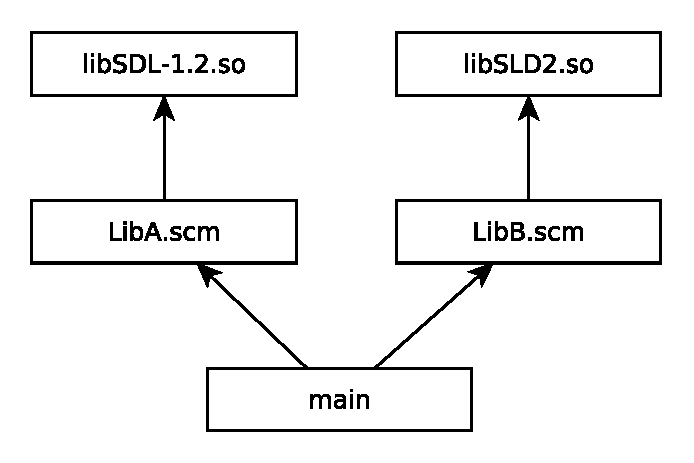
\includegraphics[width=4cm]{figures/SchemeLibrary}
%    \caption{Dépendence en diamant}
%    \label{fig:dep1}
%  \end{center}
%\end{figure}

%% NOTE: Soit P un processus, execution(A, P=[A,B]) == execution(A, P=[A]).
%Soit un processus \textbf{P} qui réfère aux bibliothèques \textbf{A} et \textbf{B}.
%Une bibliothèque peut masquer les symboles d'une autre bibliothèque chargé dans le même processus.
%La bibliothèque \textbf{A} coexiste avec la bibliothèque \textbf{B} si la \textbf{A}
%ne masque pas des symboles ne \textbf{B} qui amène un comportement non défini.


% Historiquement, il y avait un problème avec la coexistence entre deux dll sous Window. TODO: devellopper

% - Système distribué (Actor), non limité par la diversité des bibliothèque.


% TODO:
%La coexistance entre plusieurs versions d'une même bibliothèque
%===========================================================
%
% - Définition d'une bibliothèque
%   - Nom symboles:
%     - Fonction
%     - Variables global
%     - Structure de donnée
%     - Macro (Compilation)
%
%- Définition par coexistence de plusieurs bibliothèque.
%- Pourquoi est-ce utile?
%- Conditions nécessaire pour la coexistence entre plusieurs versions d'une même bibliothèque soit possible.
%  - Data race.
%  - État partagé.
%- Système d'exploitation (DOS)


\section{Conditions nécessaires}% FIXME: Pas un bon nom
Des conditions suffisantes pour que deux bibliothèques puissent coexister ensemble
dans un même processus incluant deux version de la même bibliothèque, c'est la pureté fonctionnelle des
fonctions et l'unicité des nom des fonctionnalité. La pureté fonctionnelle garantie
que chaque fonction de la bibliothèque retourne toujours le même résultat quand il
est invoqué avec les mêmes arguments sans utilisé l'affectation d'une variable globale.
Dans un contexte \textit{multi-threadé}, l'avantage principale est qu'il n'est pas possible
d'avoir une condition de course sur une donnée partagé si les fonctions sont purement fonctionnelle,
car pour qu'une condition de course se produise il faudrait un effet de bord (assignation), qui impliquerait
que la fonction n'est pas pure. Le fait que chaque fonctionnalité est associé à un nom unique cela inhibe
la capacité d'une bibliothèque de masquer une fonctionnalité d'une autre bibliothèque.

Une condition de courses
survient lorsque l'ordre des opérations d'un programme s'exécute dans un ordre
que le programmeur n'a pas conçu. Par exemple, un application avec deux fils
d'exécutions, un qui lit la valeur d'une variable globales l'autre qui l'écrit.
Deux scénarios sont possible, la lecture peut s'effectuer avant ou après la la
modification de la variable globale selon l'ordonnancement de ces deux fils d'exécution.
Le résultat de la lecture est dépendant de l'ordonnancement de ces deux opérations.

Comme mentionné ces conditions sont suffisante pour que deux bibliothèques coexiste sans problème,
mais elles ne sont non nécessaires. Il existe des bibliothèques
qui ne respect pas ces conditions, mais peuvent coexister avec d'autres
bibliothèques. Pour tester la coexistence entre plusieurs bibliothèques,
des expériences ont été effectué dans plusieurs systèmes de modules
existant. Le but de l'expérience est d'observer le bon fonctionnement
des la bibliothèques au sein de même processus.

Les expériences qui suivent permette d'observer
les caractéristiques des bibliothèques qui ne respecte pas ces conditions
qui peuvent cohabiter au sein d'une même application et aussi les
caractéristiques de ceux qui ne fonctionne pas.

% XXX
La capacité d'un langage d'interfacer avec d'autre langage via la FFI propage
les limitations du langage cible.


\subsection{Librairie C}
Les bibliothèques C sont directement compilé vers un format natif pour la plateforme courante
(e.g. Window, MacOSX, Linux). Leur format diffère d'un système d'exploitation à un autre, Window utilise le format \textit{dll}
(\textit{dynamic loading library}), MacOSX utilise le format \textit{dylib} (\textit{Mach-O dynamic library})
et Linux utilise le format \textit{so} (\textit{shared library}).

Les bibliothèques C consistent de symboles qui correspondent aux fonctions est variables
globales exportées. Une bibliothèque est généralement lié à un programme C en le spécifiant
durant la création du programme. Lors de l'exécutions les symboles non définit dans le programme
sont résolu par le \textit{dynamic linker}.

% TODO: complete
% - Bibliotheques avec collisions de nom de symboles
% - Masquage de fonctionnalité d'une des deux bibliothèque
Les collisions de symboles entre deux bibliothèques cause un masquage de
fonctionnalité d'une des deux bibliothèques. Un problème est de savoir si cela est
possible de chargé deux bibliothèque avec des collisions de symboles et accéder aux
fonctionnalités distincts de ces bibliothèques.

Pour chargé deux versions d'une même bibliothèque en C, il faut utilisé un moyen
qui prend en compte des symboles communs. La résolution des symboles ce fait
par un parcourt en largeur dans la liste des symboles des bibliothèques.
Le résultat est le premier objet qui correspond au nom de symbole recherché.
L'ordre des bibliothèques utilisé dans la résolution des symboles correspond
à l'ordre spécifié lors de la construction de l'exécutable.
%    \vspace{-10pt}
\begin{center}
\begin{figure}[ht]
\begin{lstlisting}[frame=single]
> gcc -lSDL -lSDL2 exemple.c -o exemple
> ldd ./exemple
libSDL.so => /usr/lib/libSDL.so
libSDL2.so => /usr/lib/libSDL2.so
\end{lstlisting}
\caption{Création d'un exécutable lié aux deux bibliothèques
SDL et SDL2 dans cette ordre.}
\label{fig:sdl_mask_sdl2}
\end{figure}
\end{center}
Les tests ont été effectué sur deux versions de SDL, la 1.2 et la 2, car SDL utilise
peut utilisé des ressource commune comme les évènements du clavier, la mémoire et
le GPU en utilisant OpenGL pour faire de l'affichage 2D ou 3D.
Plusieurs situations sont testés, chacune sans thread et avec des threads:
\begin{enumerate}
    \item Une utilisation de SDL minimaliste qui n'écoute pas les évènements utilisateurs.
    \item Une utilisation de SDL avec une boucle d'évènements de base.
    \item Une utilisation de SDL avec une utilisation d'un contexte OpenGL.
\end{enumerate}

%% SDL1.2 appel ces propres fonctions et SDL2 appel ces propres fonctions.
Puisque SDL1.2 et SDL2 on des collisions de symboles (i.e.\ \verb+SDL_Init+, \verb+SDL_FillRect+, \verb+SDL_BlitSurface+,
\dots), l'une des premiers observations à effectuer est la bonne répartition des appels de fonctions des deux bibliothèques
dans le contexte d'une même application. Le problème à identifier est un appels à une fonction qui est dans SDL1.2 qui est redirigé
vers SDL2. Le facteur qui influence laquelle des deux bibliothèques va masquer l'autre est l'ordre dans laquelle
ils sont lié au programme à la création, comme montré à la figure-\ref{fig:sdl_mask_sdl2}.

Le masquage amène une problématique qui peut mener à une défaillance du programme, car cela peut provoquer
la transmission d'une structure incompatible de la première bibliothèque à la deuxième. Dans le cas de SDL, la structure
\verb+SDL_Surface+ à une disposition différente des champs, donc incompatible.
Le premier champ qui décale l'alignement de ces deux structures est le \textit{pitch},
qui dans SDL1.2 est déclaré en Uint16 alors qu'en SDL2 il est un int qui sont des types de
taille différente. Donc, l'accès au prochain champ \texttt{pixels} est différent entre SDL1.2
et SDL2, ce qui peut causer un accès non désiré en mémoire si une structure de SDL1.2 est accédé comme
une structure de SDL2.
\begin{center}
\begin{tabular}{p{18em}p{18em}}
\begin{lstlisting}[frame=single,numbers=left]
typedef struct SDL_Surface {
    Uint32 flags;
    SDL_PixelFormat *format;
    int w, h;
    Uint16 pitch;
    // Different offset here
    void *pixels;
    ...
} SDL_Surface;
\end{lstlisting}&
\begin{lstlisting}[frame=single,numbers=right]
typedef struct SDL_Surface {
    Uint32 flags;
    SDL_PixelFormat *format;
    int w, h;
    int pitch;
    // Different offset here
    void *pixels;
    ...
} SDL_Surface;
\end{lstlisting}\\
\end{tabular}
\end{center}
%% Instable: gcc -lSDL -lSDL2 ...
Puisque les programmeurs cherchent une certaine stabilité dans leurs bibliothèques, ils ont
tendance à éviter les dépendances avec des bibliothèques qui ont des collisions de fonctionnalités.
Il est peut probable d'avoir une cohabitation entre deux bibliothèques avec des nom de fonctionnalités
similaires lié à un programme où bibliothèque par des arguments du compilateur.

Le cas qui pourrait permettre plusieurs bibliothèques avec des collisions de symboles
au sein d'une même est avec l'API du \textit{dynamic linker}. Un teste simple permet
de démontrer la capacité de répartir les appels d'une fonction identifié par le même nom
dans différentes bibliothèques.

La structure générale des tests est organisé comme suit. Deux bibliothèques implémentant
une interaction valide avec l'une des versions de la bibliothèque (e.g. SDL1.2, SDL2).
Un application qui unie ces deux bibliothèques en utilisant l'API du
\textit{dynamic linker} pour exécuter ces deux bibliothèques séquentiellement ou
parallèlement.

%% TODO: expliquer la structure des programmes.

Dans le test minimaliste sans gestion d'évènements l'exécution des bibliothèque
fonctionne dans les deux cas, séquentiellement et en parallèle. La raison qui
explique ce bon fonctionnement est la répartition des appels au fonctions
des deux bibliothèques et le fait qu'il n'utilise pas de structure commune,
qui pourrait causer des conditions de course dans le test en parallèle.

\begin{center}
  \begin{figure}[ht]
\begin{lstlisting}[language=C,frame=single]
#include <SDL/SDL.h>

int main(int argc, char **argv) {
  SDL_Init(SDL_INIT_VIDEO);
  SDL_WM_SetCaption("sdl1_2", NULL);
  SDL_Surface *win =
    SDL_SetVideoMode(200, 200, 24, SDL_HWSURFACE);

  Uint32 color = SDL_MapRGB(win->format, 255, 0, 0);

  SDL_FillRect(win, NULL, color);
  SDL_Flip(win);
  SDL_Delay(1000);

  SDL_FreeSurface(win);
  SDL_Quit();
  return 0;
}
\end{lstlisting}
    \caption{Programme qui utilise la bibliothèque SDL1.2 sans la gestion des évènements
    Cette application génère une fenêtre rouge qui se ferme après 1 seconde de délais.}
  \end{figure}
\end{center}

%TODO: wrap these into frame
\begin{center}
  \begin{figure}[ht]
\begin{lstlisting}[language=C,frame=single]
#include <SDL2/SDL.h>

int main(int argc, char **argv) {
  SDL_Init(SDL_INIT_VIDEO);
  SDL_Window *win = SDL_CreateWindow("title",
      SDL_WINDOWPOS_CENTERED, SDL_WINDOWPOS_CENTERED,
      200, 200, SDL_WINDOW_SHOWN);
  SDL_Surface *screen = SDL_GetWindowSurface(win);

  Uint32 color = SDL_MapRGB(screen->format, 0, 255, 0);
  SDL_FillRect(screen, NULL, color);
  SDL_UpdateWindowSurface(win);
  SDL_Delay(1000);
  SDL_DestroyWindow(win);
  SDL_Quit();
  return 0;
}
\end{lstlisting}
    \caption{Programme qui utilise la bibliothèque SDL2 sans la gestion des évènements.
    Cette application génère fenêtre verte qui se ferme aussi après 1 seconde de délais.}
  \end{figure}
\end{center}

Dans le test incluant des évènements, l'hypothèse supposait que les évènements du clavier
aurait causé des problèmes de conditions de course en parallèle. Le test a aussi fonctionné
séquentiellement et en parallèle, malgré la dépendance commune du clavier.

Le test qui incluait OpenGL, n'aurait pas dû fonctionné par hypothèse. Les deux version
de SDL référait à une unique version de OpenGL. Le résultat a été surprenant, car le test
séquentielle et parallèle à fonctionné. Ce qui amène à conclure qu'il existe des cas
de coexistence entre des bibliothèques avec des collisions de symbole qui fonctionne
sans causer des problèmes d'exécution.



%%% Possible de compile le programme principale en un exécutable et en bibliothèque.
%Les deux programmes sont compilés en bibliothèques et en exécutables.
%Le fonctionnement de chaque programme est testé de façon séparé.
%Le programme principale, qui charge le main des deux autres programmes en utilisant
%l'API du \textit{dynamic loader}, est compilé en mode séquentiel et en mode parallèle.
%La version séquentielle permet d'observer la coexistance entre les deux bibliothèques,
%celle parallèle est utilisé pour évaluer les conditions de course sur des ressources
%communes.
%
%%% TODO: schema.
%\begin{center}
%  \begin{figure}[ht]
%\begin{lstlisting}[language=C,frame=single]
%  ...
%  void *hndl1 = dlopen(prog1, RTLD_NOW);
%  void *hndl2 = dlopen(prog2, RTLD_NOW);
%
%  int(*main1)(int,char**) = dlsym(hndl1, "main");
%  int(*main2)(int,char**) = dlsym(hndl2, "main");
%
%  main1(argc, argv);
%  main2(argc, argv);
%  ...
%\end{lstlisting}
%  \caption{Le chargement et exécution séquentiel de la fonction main des programmes
%  \textbf{prog1} et \textbf{prog2} via l'API du \textit{dynamic loader}.}
%  \end{figure}
%\end{center}
%% \begin{center}
%%   \begin{figure}[ht]
%% \begin{lstlisting}[language=C,frame=single]
%% struct MainCallback {
%%   int argc;
%%   char **argv;
%%   int (*main)(int,char**);
%% };
%%
%% void *run(void* args) {
%%   struct MainCallback* callback = (MainCallback*)args;
%%   callback->main(callback->argc, callback->argv);
%%   return NULL;
%% }
%% \end{lstlisting}
%%   \caption{Callback utilisé pour exécuté le main de la bibliothèque chargé par
%%   \textbf{dlsym} en parallèle avec pthread.}
%%   \end{figure}
%% \end{center}
%
%\begin{center}
%  \begin{figure}[ht]
%\begin{lstlisting}[language=C,frame=single]
%  ...
%  struct MainCallback callback = {
%    .argc = argc,
%    .argv = argv,
%    .main = main1
%  };
%
%  pthread_t th1;
%  pthread_create(&th1, NULL, run, &callback);
%  main2(argc, argv);
%  pthread_join(th1, NULL);
%  ...
%\end{lstlisting}
%    \caption{Exécution du code des deux programme en parallèle avec l'utilisation de pthread.
%    Contrairement à la figure précédente, la fonction main de \textbf{prog1} exécuté dans un
%    threads.}
%  \end{figure}
%\end{center}
%
%
%Tout d'abord, la compatibilité entre SDL1.2 et SDL2 à été testé par un code sans
%la gestion des évènements, pour vérifier si les fonctions respective de chaque
%bibliothèque étaient à appellé correctement.
%% coexistance sans interraction directe.
%#ifdef THREADED

% SDL1.2/SDL2/OpenGL
% - Hypothèse
%   - Non-threaded without OpenGL
%   - Non-threaded with OpenGL
%   - Threaded without OpenGL
%   - Threaded with OpenGL
% - Démarche
% - Résultat
% - Petite Conclusion

% OpenSSL+RSA/OpenSSL+Socket
% - Hypothèse
% - Démarche
% - Résultat
% - Petite Conclusion

\clearpage
\subsection{Bibliothèque Scheme}
La compatibilité entre version a été testé sur la partie cryptographique
RSA de OpenSSL, SDL et un générateur aléatoire qui possède un état global.
Pour testé les bibliothèques natives en Scheme, il a fallut écrire des
bibliothèque Scheme contenant des déclarations de type et des déclarations de
fonctions qui lient le code natif au monde Scheme.

Par hypothèse la partie cryptographique des deux versions de OpenSSL peuvent
coexister. Chacune des fonctions cryptographique de OpenSSL1.0 et OpenSSL1.1
exécute du code disjoint qui n'interfère pas avec une zone mémoire commune.
Cela implique qu'un appelle à une fonction de OpenSSL1.0 n'affectera pas les
résultats des appelles futures de OpenSSL1.1. Les fonctions nécessaires
pour tester la partie cryptographique RSA sont:
\begin{itemize}
    \item \lstinline{PEM_read_bio_RSA_PUBKEY} et \lstinline{PEM_read_bio_RSAPrivateKey}:
        Ce sont les fonctions OpenSSL qui permettent de lire la clef publique et la clef privée.
    \item \lstinline{RSA_public_encrypt}:
        La fonction d'encryption qui crypte un  message en utilisant une clef publique.
    \item \lstinline{RSA_private_decrypt}:
        La fonction qui permet de décrypter un message en utilisant la clef privée.
    \item \lstinline{RSA_free}:
        La fonction qui libère la mémoire alloué pour les clefs publiques et privées.
        Cette fonction n'est pas nécessaire pour les testes, mais utile pour une bonne
        gestion mémoire.
\end{itemize}
La structure de donnée utilisé par les fonctions d'OpenSSL pour la cryptographie RSA
est un pointeur vers un enregistrement RSA. La liaison avec le type C est effectué avec
la forme spécial \lstinline{c-define-type}.

Le teste consiste à crypter un message en utilisant une clé publique, décrypter le
cryptogramme avec la clé privée et comparer le message original avec le message décrypter
pour les deux versions de OpenSSL chargé dans le même processus. Pour vérifier la bonne
invocation des fonctions de OpenSSL1.0 et OpenSSL1.1 respectif le débogueur \textbf{gdb}
a été utilisé. Les bibliothèques d'OpenSSL consiste en deux fichier \url{libssl.so} et \url{libcrypto.so}.
En déboguant la répartition des appels avec \textit{gdb}, il y a eu l'observation que 
la bibliothèque \url{libcrypto.so} de OpenSSL1.1 masquait la version de OpenSSL1.0 s'il
n'est pas spécifié explicitement lors de la création de la bibliothèque Scheme \textit{rsa.scm}
comme à la figure-\ref{fig:scm_masq1}. Les raisons sont liées à plusieurs facteurs qui étaient présents
durant l'expérience. L'ordre de recherche des symboles qui inclue les symboles des bibliothèques lié à
l'exécutable qui sont prioritaire qui contenait \url{libssl.so} et \url{libcrypto.so} de OpenSSL1.1.
Dans ce cas, il était possible de résoudre ce problème en ajoutant une
dépendance directe à \texttt{libcrypto} lors de la construction des bibliothèques Scheme \verb+RSA+
comme montré dans la figure-\ref{fig:scm_masq_fix1}.

\begin{center}
\begin{figure}[ht]
\begin{lstlisting}[frame=single]
gsc-script -o rsa-1-0-0.o1 \
  -cc-options '-I /usr/include/openssl-1.0' \
  -ld-options '-L /usr/lib/openssl-1.0 -lssl' \
  -prelude '(define-cond-expand-feature|openssl-v10|)' rsa.scm

gsc-script -o rsa-1-1-0.o1 \
  -ld-options "-lssl" rsa.scm
\end{lstlisting}
\caption{Création des bibliothèques \textit{rsa.scm} pour OpenSSL1.0 et OpenSSL1.1
sans la spécification de \textit{libcrypto.so}}
\label{fig:scm_masq1}
\end{figure}
\end{center}

\begin{center}
\begin{figure}[ht]
\begin{lstlisting}[frame=single]
gsc-script -o rsa-1-0-0.o1 \
  -cc-options '-I /usr/include/openssl-1.0' \
  -ld-options '-L /usr/lib/openssl-1.0 -lssl -lcrypto' \
  -prelude '(define-cond-expand-feature|openssl-v10|)' rsa.scm

gsc-script -o rsa-1-1-0.o1 \
  -ld-options "-lssl -lcrypto" rsa.scm
\end{lstlisting}
\caption{Création des bibliothèques \textit{rsa.scm} pour OpenSSL1.0 et OpenSSL1.1
avec la spécification de \textit{libcrypto.so}}
\label{fig:scm_masq_fix1}
\end{figure}
\end{center}

\begin{center}
\begin{figure}[ht]
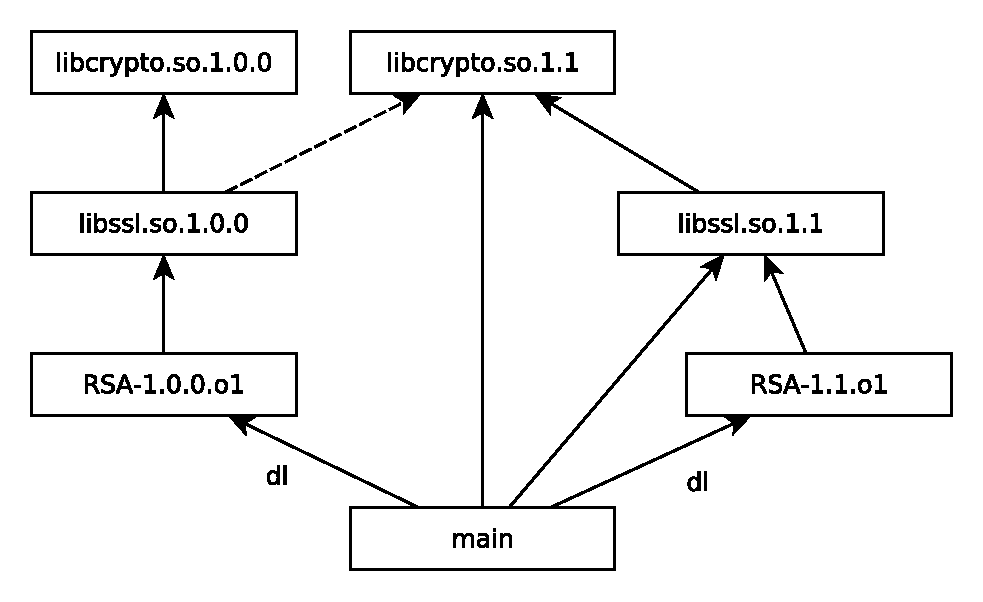
\includegraphics{figures/libssl_masking.pdf}
\caption{Schéma qui montre les dépendances entre les bibliothèques au sein du processus.
Les dépendances qui ont été lié dynamiquement lors la création de l'application sont représenté par une flèche avec
trait plein sans annotation. Ceux qui représente les chargement de bibliothèque dynamique manuellement ont
l'annotation \textit{dl}. La flèche en pointillé indique un masquage des symboles de la bibliothèque
source par celle pointée.}
\label{fig:scm_masq_schema}
\end{figure}
\end{center}


TODO: rng générator

%\begin{lstlisting}[frame=single]
%(c-define-type RSA* (pointer "RSA"))
%\end{lstlisting}


%Heureuse Gambit Scheme possède un interface pour lié
%une fonction C au monde Scheme.

%Une bibliothèque liant les fonctions principales de SDL au monde Scheme.


\TODO{Fill}
% SDL / SDL2
% - Hypothèse
% - Démarche
% - Résultat
% - Petite Conclusion

% OpenSSL+RSA
% - Hypothèse
% - Démarche
% - Résultat
% - Petite Conclusion

% RNG-splitmx64/RNG-xoroshiro128+
% - Hypothèse
% - Démarche
% - Résultat
% - Petite Conclusion


\subsection{Bibliothèque Javascript (NodeJS)}
\TODO{Fill}
% Démarche général
% express / sqlite3
% - Hypothèse * 2
% - Démarche/Expérimentation
% - Résultat
% - Petite Conclusion

Pour effectué des tests sur la coexistences de différente version d'une bibliothèque
Javascript dans NodeJS, il faut tout d'abord permettre l'importation de plusieurs
versions d'une même bibliothèque. Dans NodeJS, l'importation de module s'effectue
avec la fonction \verb|require(module-name)|. Puisque l'information de version
de la bibliothèque n'est pas fournit en paramètre à la fonction, il faut donc
utilisé une autre méthode de forcer plusieurs versions des bibliothèque.
La configuration d'un module dans NodeJS utilise le format JSON pour spécifier
le nom, la version, les dépendances, \dots.

Les dépendances sont conservées sous la forme d'un arbre, chaque module à ses dépendances directes
qui ont aussi des dépendances indirectes.  Lors de l'écriture d'un module Javascript, il est possible
de spécifier la version de chaque dépendence dans le fichier \textit{package.json}.
\begin{verbatim}
{
  ...
  "dependencies": {
    "express": "4.16.3"
  },
  ...
}
\end{verbatim}
En utilisant cette fonctionnalité du système de module de NodeJS, deux bibliothèques \textit{wrapper}
sont écrit pour interfacer les deux versions de express. Puisque l'API public d'express n'a pas changé entre
les versions 3.21.1 et 4.16.3, il est possible de recycler le code de la bibliothèque qui encapsule une
version d'express (figure-\ref{fig:express}).
\begin{center}
\begin{figure}[ht]
    % FIXME: language=Javascript
    \begin{lstlisting}[language=C,frame=single]
const express = require('express');

function start() {
  const app = express();
  const port = Math.floor(Math.random() * 64535 + 1000);

  app.get('/', (req, res) => {
    res.send('Hello world!\n');
  });

  app.listen(port, 'localhost', () => {
    console.log('Listen on port ' + port);
  });
}
exports.start = start;
\end{lstlisting}
\end{figure}
\label{fig:express}
\end{center}
Le programme principale ne fait qu'importer les deux encapsulation de bibliothèque
et invoque la fonction \textit{start}.

Le résultat attendu dans cette expérience est que ces deux version de la bibliothèque
express coexiste sans problème, sauf dans le cas où le port tcp utilisé par les deux
version est le même. Dans ce cas, c'est la bibliothèque dont la fonction
\textit{start} a été invoqué en premier qui va monopoliser le tcp port. Dans ce cas
la ressource qui inhibe la coexistence de ces modules au sein d'un même processus
est lié au \textit{socket}.

\subsection{Variables globales communs}

Puisque qu'il n'existe qu'une seul instance de chaque bibliothèque en mémoire, cela implique
que les variables globale d'une bibliothèque.

Définissons 3 bibliothèques B, C et D telle que D a une variable globale nommée \textit{value}.
B et C ont chacun une dépendance directe vers D, et exportent une référence de la variable
globale \textit{value} de D.

Le programme principale A commence par charger B et C. Ensuite lit la valeur de \textit{B.D.value}
puis modifie \textit{C.D.value} et relit \textit{B.D.value}. Le teste réussi si la valeur de
\textit{B.D.value} reste inchangé par la modification de \textit{C.D.value}. Cela implique que
les références vers la bibliothèque D est différente de via B et via C.

Dans NodeJS, un module peut être installé via un dossier, un archive tarball, un dépôt de code source git ou
directement via Npmjs. Puisque un module publié dans Npmjs ne peut pas être retiré facilement étant donné
la politique lié au module (\url{https://docs.npmjs.com/cli/unpublish}).
%L'expérience va utilisé un serveur git qui est auto-hébergé.


%\section{Section un du chapitre un}
%\textbf{texte\dots}
%
%\subsection{Sous-section un}
%texte\dots
%\begin{itemize}
%\item   item 1.
%\item   item 2.
%\end{itemize}
%
%\subsubsection{Sous-Sous-section un}
%texte\dots
%
%\subsection{Sous-section deux}
%texte\dots
% \begin{gather}
%   4+5
% \end{gather}
%\begin{enumerate}
%\item item 1 avec numérotation.
%\item item 2 avec numérotation.
%\end{enumerate}
%
%Une définition.
%\begin{deff}[Une définition]
%  Une définition.
%\end{deff}
%et un théorème
%\begin{theo}[Titre]
%  Ceci est vrai!
%\end{theo}
%\begin{proof}
%  et voici la preuve en ``majuscules''.
%\end{proof}
%
%\begin{demo}
%  et voici la preuve en gras.
%\end{demo}
%
%Pour obtenir le résultat précédent (Démonstration en gras), nous aurions pu taper
%\begin{verbatim}
%\renewcommand{\proofname}{\textbf{Démonstration}}
%\end{verbatim}
%dans le préambule (avant le \verb|\begin{document}|).

%%
%% Nous passons une page...
%%
\newpage

%%
%% On peut citer un livre:
%%

%Citons un livre\dots voir~\cite{ams:guide}.

%%
%% Voici trois types d'insertion de figures.
%%

%\vspace{2cm}
%\noindent\centerline{\tt Pour voir des exemples d'insertions d'images,}
%\noindent\centerline{\tt enlevez les commentaires ici dans le \.tex.}
%Voici une insertion simple:
% \begin{figure}[ht]
%   \begin{center}
%     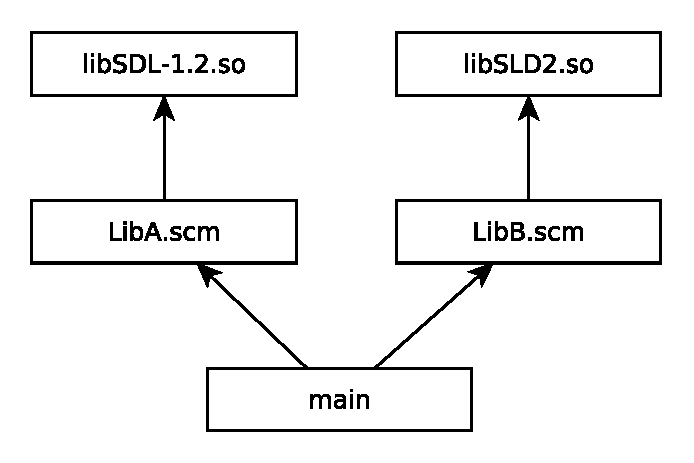
\includegraphics[width=4cm]{figures/SchemeLibrary}
%     \caption{Scheme}
%     \label{fig:1}
%   \end{center}
% \end{figure}
%%
%%Voici une insertion de plusieurs figures:
%%\begin{figure}[ht]
%%  \begin{center}
%%    \subfigure[Un cercle.]{\label{fig:2} 
\includegraphics[angle=-90,
%%      width=2.9cm]{figures/cercle}} \hspace{2cm}
%%    \subfigure[Un carré.]{\label{fig:3} 
\includegraphics[angle=-90,
%%      width=2.9cm]{figures/carre}}
%%    \caption{Des figures}
%%    \label{fig:4}
%%  \end{center}
%%\end{figure}

%%--------------%
%%     index    %
%%--------------%

%% S'il y a lieu, décommenter la ligne pour mettre votre index

%%\printindex

%%------------------------------------------------- %
%%         références --- bibliographie             %
%%------------------------------------------------- %

%\bibliographystyle{plain-fr}
%\bibliography{<fichier.bib>}

%\begin{thebibliography}{DDDD}
%
%\bibitem[A]{ams:guide}
%  {\scshape American Mathematical Society},
%  \emph{\AmS\LaTeX{} Version 1.1 User's Guide},
%  Amer. Math. Soc., Providence, R.~I., 1991.
%
%\bibitem[GMS]{latex2e:1}
%{\scshape M. Goossens, F. Mittelbach, and A. Samarin},
%\emph{The \LaTeX{} companion},
%Addison-Wesley, USA, 1994.
%
%\bibitem[H]{hahn:everyone}
%{\scshape J. Hahn},
%\emph{\LaTeX{} for Everyone: A reference guide and tutorial for
%    typesetting documents using a computer},
%     Personal \TeX, Inc., Mill Valley, CA., 1991.
%
%\bibitem[L]{lamport:latex}
%{\scshape Leslie Lamport},
%\emph{\LaTeX{} -- A Document Preparation System},
%     Addison-Wesley, Reading, Mass., 1986.
%
%\bibitem[M]{mckay:sty}
%{\scshape W. McKay},
%\emph{udemmem-l.sty}, fichier \LaTeX,  rédigé pour le compte de
%l'Université de Montréal, 1993.
%
%\bibitem[S]{spivak:joy}
%{\scshape M. D. Spivak},
%\emph{The Joy of \TeX{}}, second edition,
%     Amer. Math. Soc., Providence, R.~I., 1990.
%
%\bibitem[T]{latex2e:2}
%{\scshape \TeX{} User Group},
%\emph{\LaTeX2e for classand package writers},
%1995, disponible sur le web.
%
%\end{thebibliography}

%%------------------------------------------------- %
%%                  Annexe A                        %
%%------------------------------------------------- %

\appendix
%\chapter{Le titre}
%
%\section{Section un de l'Annexe A}
%
%texte
%
%\chapter{Les différentes parties et leur ordre d'apparition}
%
%J'ajoute ici les différentes parties d'un mémoire ou d'une thèse ainsi
%que leur ordre d'apparition tel que décrit dans le guide de
%présentation des mémoires et des thèses de la Faculté des études
%supérieures.  Pour plus d'information, consultez le guide sur le site
%web de la facutlé (www.fesp.umontreal.ca).
%
%\begin{table}[htbp]
%  \begin{center}
%    \begin{tabular}{|lr|}\hline
%      1. les couvertures conformes & obligatoires\\
%      2. les pages de garde & obligatoires\\
%      3. la page de titre & obligatoire\\
%      4. l'identification du jury& obligatoire\\
%      5. le résumé en français et les mots clés français& obligatoires\\
%      6. le résumé en anglais et les mots clés anglais & obligatoires\\
%      8. le résumé de vulgarisation& facultatif\\
%      9. la table des matières, la liste des tableaux,\phantom{un fantome d'espace}&\\ \phantom{9. } la liste des figures & obligatoires\\
%      10. la liste des sigles, la liste des abréviations& obligatoires\\
%      11. la dédicace& facultative\\
%      12. les remerciements & facultatifs\\
%      13. l'avant-propos & facultatif\\
%      14. le corps de l'ouvrage& obligatoire\\
%      15. l'index analytique& facultatif\\
%      16. les sources documentaires & obligatoires\\
%      17. les appendices (annexes) & facultatifs\\
%      18. le curriculum vitæ & facultatif\\
%      19. les documents spéciaux & facultatifs\\\hline
%    \end{tabular}
%    \caption{Liste des parties}
%  \end{center}
%\end{table}

\end{document}
